\section{Introduction}

Most Chip Multiprocessors (CMPs) share parts of the memory system to improve resource utilization.
In particular, the last level cache (LLC) is commonly shared between processor cores.
This design choice makes destructive cache interference possible which reduces performance and may cause problems such as missed deadlines, priority inversion, unpredictable interactive performance and non-compliance with service level agreements \cite{dubois13}.
For this reason, computer architecture researchers have proposed a large number of microarchitectural techniques that partition the LLC between competing processes \magnus{add long list of citations}.
Given the large amount of cache partitioning research, it is common to reuse previously proposed ideas in new schemes.
Unfortunately, it can be hard to identify this reuse without understanding the work in detail.
In this work, we systematically analyze the cache partitioning research field and identify overlap with the aim of helping future architects avoid reinventing the wheel.

We loosely define the cache partitioning problem as the task of managing shared LLC capacity in a thread-aware manner with the aim of achieving a performance-related goal.
We differentiate between \textit{explicit} and \textit{implicit} cache partitioning.
In explicit cache partitioning, each running process is assigned an LLC quota which determines the minimum amount of cache space the process will have \magnus{add references to examples}.
With implicit partitioning, LLC space is managed by process-aware LLC policies without assigning a specific quota to each process \magnus{add references to examples}.

The first contribution of this work is a classification of previously proposed cache partitioning techniques.
All cache partitioning techniques contain a \textit{policy} which defines the goal to be achieved with partitioning and \textit{mechanisms} that are the primitives used to implement the policy \cite{virtualPrivateMachines}.
The two most common policies are to minimize the total number of LLC misses or to provide \textit{Quality of Service (QoS)} by ensuring that the performance of one or more processes is kept above a certain level.
Cache partitioning techniques also commonly use a \textit{feedback} mechanism and a \textit{partitioning} mechanism.
\magnus{Will splitting the partitioning mechanism into partitioning and enforcement simplify the arguments?}
The feedback mechanism gathers information regarding the cache requirements of the currently running processes while the partitioning mechanism is used to select and enforce partitions (explicitly or implicitly).
Examples of feedback mechanisms are \textit{Auxilliary Tag Directories (ATDs)} \cite{utilityBasedCachePartitioning,haakonHiPC} and marginal gain counters \cite{dynPartofSharedCacheMemory,suh02} and examples of partitioning mechanisms are way partitioning  \cite{utilityBasedCachePartitioning} and modified promotion and insertion policies (e.g.\ \cite{xie09}).

The main observation resulting from this classification is that almost all proposed cache partitioning techniques apply previously proposed ideas in some form.
For instance, the ATD feedback mechanism has been used extensively \magnus{add complete list of citations}.
This is not surprising given the large number of proposed techniques targeting cache partitioning, but for science to progress it is critical that these overlaps are clearly identified.
This work is to the best of our knowledge the first to systematically classify the policies and mechanisms used in previous cache partitioning schemes.
Thus, our classification scheme enable architects to clearly separate their novel ideas from previous work.

The second contribution of this work is a quantitative instigation of the performance of 5 high-impact cache partitioning techniques that collectively cover the current design space of miss minimizing partitioning techniques targeted at monolithic LLCs \magnus{verify that this is correct}.
Concretely, we implemented TADIP \cite{jaleel08}, DRRIP \cite{jaleel10}, UCP \cite{utilityBasedCachePartitioning}, PIPP \cite{xie09} and PriSM \cite{manikantan12}.
The baseline is a conventional LRU-managed shared LLC.
\magnus{What did we find?}
\magnus{Add the progression over time plot here?}
We aim to provide our implementations to the research community.

\magnus{Add outline of the work? Do we need it?}

% Previous "meta analyses", can we get them in somewhere: \cite{microlib,comparingPrevalingSimulationTechniques,desmet10}).

\section{Cache Partitioning Techniques}

\begin{table*}[tp]
	\caption{Cache Partitioning Technique Overview}
	\label{tab:cachePartTaxonomy}
	\begin{tabularx}{\textwidth}{llcXXX}
	\toprule
	Year & Scheme & Ref. & Policy & Feedback Mechanism & Partitioning Mechanism \\	
	\midrule
	2000 & Column Caching & \cite{columnCaching} & - & - & Column caching (first) \\
	2002 & Suh et al. & \cite{suh02,dynPartofSharedCacheMemory} & Global miss minimization & Marginal gain counters (first) & Cache quota partitioning (first?) \\
	2004 & Kim et al. & \cite{fairCacheSharingAndPartitioning} & Fairness & Marginal gain counters & Cache quota partitioning LRU \\
	2004 & CQoS & \cite{cqos} & Priority-based & - & Set partitioning, selective cache allocation and heterogeneous cache regions \\
	2006 & Utility Based Cache Partitioning (UCP) & \cite{utilityBasedCachePartitioning} & Global miss minimization & Auxiliary Tag Directory (ATD) & Way Partitioning \\ 
	2006 & Dybdahl et al. & \cite{haakonHiPC} & Global miss minimization & ATD (called shadow tags) & Way partitioning \\
	2006 & Settle et al. & \cite{dynReconfCache} & Reuse-based heuristics & Access and reuse counters & Column caching and LRU heuristic \\
	2006 & Rafique et al. & \cite{osSupportForFairCacheSharing} & OS-based priorities and miss-rate equalization \cite{fairCacheSharingAndPartitioning} & Marginal gain counters and IPC & Way partitioning \\
	2006 & Hsu et al. & \cite{sharedCachePolicies} & Equal share (Communist) and maximum total benefit (Utilitarian) & - & - \\
	2006 & STATSHARE & \cite{petoumenos06} & OS: Minimize miss rate, maximize "usefulness", QoS  & Sampled, quantized reuse-distance histograms  & Replace decayed over non-decayed cache lines randomly\\
	2007 & Cooperative Cache Partitioning (CCP) & \cite{cooperativeCachePartitioning} & Fair speedup and weighted speedup & - & Time-sharing \\
	2007 & Guo et al. & \cite{qosInCMPs} & QoS with admission policy, resource stealing and speculative downgrade  & ATD & Way partitioning \\
	2007 & Virtual Private Caches (VPC) & \cite{virtualPrivateCaches} & QoS with IPC targets, fairness policy distributes left-over resources & - & VPC Arbiter (based on network fair queuing) and VPC Capacity Manager (way partitioning) \\
	2007 & Thread-Aware Dynamic Insertion Policy (TADIP) & \cite{jaleel08} & Global miss rate minimization & Set dueling \cite{shadowTagInsertionPolicies} & TADIP \\
	2007 & Iyer et al. & \cite{qosPoliciesForCMP} & QoS: Static vs.\ dynamic & Shared unit utilization & Cache quota partitioning per QoS-level \\
	2009 & FlexDCP & \cite{flexDCP} & OS-guided performance fairness & ATD & Column caching \\
	2009 & Zhou et al. & \cite{zhou09} & Performance fairness (identical slowdowns) & Overlap counters and ATD & Overalloc counter and modified LRU \\
	2009 & Promotion/Insertion Pseudo-Partitioning (PIPP) & \cite{xie09} & Global miss minimization & ATD & PIPP \\
	2009 & SHARP Control & \cite{sharpControl} & Fair speedup and QoS & IPC target and miss rate models are input & Way partitioning \\
	2010 & Re-Reference Interval Prediction (RRIP) & \cite{jaleel10} & Global miss minimization & Set Dueling (for DRRIP and TA-DRRIP) & SRRIP, DRRIP and TA-DRRIP replacement policies \\
	2010 & Yu et al. & \cite{yu10} & Off-chip bandwidth minimization & Off-line profiling & Set partitioning \cite{ranganathan00}  \\
	2010 & Xie et al. & \cite{xie10} & \toni{Fill out if needed} & & \\
	2011 & Wang et al. & \cite{wang11} & Meet deadlines and minimize energy & Off-line profiling & Static way partitioning \\
	2011 & NUcache & \cite{manikantan11} & Minimize global miss rate & DeliTrack and NUTrack & NUcache \\
	2011 & Vantage & \cite{sanchez11} & Global miss minimization & ATD & Vantage \\
	2012 & Cooperative Partitioning & \cite{sundararajan12} & Power-directed global miss minimization & ATD & Column caching variant for energy reduction \\
	2012 & PriSM & \cite{manikantan12} & Global miss minimization, fairness and QoS & ATD and counters & PriSM \\
	2012 & Duong et al. & \cite{duong12} & Global miss minimization & Reuse distance distributions &Protecting Distance replacement \\
	2012 & Hasenplaugh et al. & \cite{hasenplaugh12} & Global miss minimization, IPC and QoS  & Gradient regions & Adaptive insertion policy \\
	2013 & Albericio et al. & \cite{albericio13} & Global miss minimization (inclusive caches) & Reused bits and beeing-used bits & Least Recently Reused and Not Recently Reused \\
	\bottomrule
	\end{tabularx}	
\end{table*}

\textit{Note: Table \ref{tab:cachePartTaxonomy} is copy pasted from my previous manuscript and will have to be modified or possibly removed.}

\runar{Add a condensed version of your background chapter here}

\begin{table*}[tp]
	\caption{Overview of Dynamic Miss Minimizing Cache Partitioning Techniques}
	\label{tab:cachePartTaxonomy}
	\begin{tabularx}{\textwidth}{lcXXXX}
	\toprule
	Year & Citations & Scheme & Feedback Mechanism & Partitioning Mechanism \\	
	\midrule
	2002 & & Suh et al.\ \cite{suh02,dynPartofSharedCacheMemory} & Marginal gain counters & Cache quota partitioning \\	
	2006 & & Utility Based Cache Partitioning (UCP) \cite{utilityBasedCachePartitioning} & Auxiliary Tag Directory (ATD) & Way Partitioning \\ 
	2006 & & Dybdahl et al.\ \cite{haakonHiPC} & ATD (called shadow tags) & Way partitioning \\
	2007 & & Thread-Aware Dynamic Insertion Policy (TADIP) \cite{jaleel08} & Set dueling \cite{shadowTagInsertionPolicies} & TADIP \\
	2009 & & Promotion/Insertion Pseudo-Partitioning (PIPP) \cite{xie09} & ATD & PIPP \\
	2010 & & Re-Reference Interval Prediction (RRIP) \cite{jaleel10} & Set Dueling (for DRRIP and TA-DRRIP) & SRRIP, DRRIP and TA-DRRIP replacement policies \\
	2010 & & Xie et al.\ \cite{xie10} & ATD (called shadow tags) & Thrasher caging (way partitioning) \\
	2011 & & NUcache \cite{manikantan11} & DeliTrack and NUTrack & NUcache \\
	2011 & & Vantage \cite{sanchez11} & ATD & Vantage \\
	2012 & & Cooperative Partitioning \cite{sundararajan12} & ATD & Column caching variant for energy reduction \\ % Power-directed global miss minimization
	2012 & & PriSM \cite{manikantan12} & ATD and counters & PriSM \\ % Global miss minimization, fairness and QoS 
	2012 & & Duong et al.\ \cite{duong12} & Reuse distance distributions &Protecting Distance replacement \\
	2012 & & Hasenplaugh et al.\ \cite{hasenplaugh12}  & Gradient regions & Adaptive insertion policy \\ % Global miss minimization, IPC and QoS
	2013 & &  Albericio et al.\ \cite{albericio13}  & Reused bits and beeing-used bits & Least Recently Reused and Not Recently Reused \\ % Global miss minimization (inclusive caches)
	\bottomrule
	\end{tabularx}	
\end{table*}


\toni{Add the missing works to Table \ref{tab:cachePartTaxonomy}}

\toni{Can you retrieve the number of citations of each global miss minimizing work from Google Scholar?
The older techniques we have implemented are likely cited a lot and then we can argue for why we selected the less cited works.}

\runar{In this section, we should discuss only the works from \ref{tab:cachePartTaxonomy}. Can you update the following sections accordingly and identify any missing discussions?}

\magnus{Write a paragraph justifying why we chose the five partitioning techniques that we did out of the at least 14 possibilities in the new Table \ref{tab:cachePartTaxonomy}}

\magnus{When the classification is complete, group works according to explicit/implicit and optimize the table wrt area}

\subsection{Implicit Cache Partitioning Techniques}

\subsubsection{LRU}

Least Recently Used (LRU) replacement, or some simplification of LRU, is one of the dominant cache management algorithms in hardware today. 
As a result, LRU is normally used as the baseline for comparisons when presenting new cache management algorithms~\cite{Jaleel2010,Qureshi2006,Qureshi2007}.

The LRU algorithm relies on temporal locality of cache accesses; recently accessed data will have a higher chance of reuse than less recently used data.
Theoretically one can envision a cache set managed by LRU as a stack, where recently accessed cache blocks are near the top and less recently accessed blocks are near the bottom.
The bottom position of the stack is the LRU position, and the top position is the MRU position.
The replacement policy of LRU is to evict the least recently used cache block, the one on the bottom of the LRU stack.
The insertion and promotion policy of LRU is the same; a inserted or accessed block is always moved to the MRU position unless it is already there.
In a hardware implementation, the blocks are not stored in a sorted fashion, but additional storage bits are used to keep track of LRU positions.

An important consequence of the LRU algorithm is that it satisfies the \textit{stack property}.
Considering two LRU managed caches, with 4- and 3-ways.
If both caches handle the same memory sequence, we know that the state of the upper three ways in both caches will be identical.
This because new and promoted blocks always enter at the top of the stack, and only the block at the bottom of the stack will be evicted.
Several algorithms make use of this property to count the number of cache misses in LRU managed caches of varying size.
In a 4-way cache, if we count the number of accesses to blocks at each way we can deduce the number of misses of any cache smaller than 4-ways. 
For a 3-way cache, the number of misses is the same as the number of misses in the 4-way cache plus the number of accesses to the fourth way.

\subsubsection{DIP}

Dynamic Insertion Policy (DIP)~\cite{Qureshi2007} was originally proposed in 2007.
Like LRU, the DIP algorithm view the cache set as a stack.
Replacement and promotion policies are equal to LRU.
Two distinct insertion policies, LRU Insertion Policy (LIP) and Binominal Insertion Policy (BIP), are used.
LIP inserts new blocks at the MRU position.
BIP inserts new blocks either at the LRU position or with a small probability, $p = \frac{1}{32}$, at the MRU position. 
The overall DIP algorithm switch between the two insertion policies attempting to always use the one that is expected to cause fewer cache misses.

By mostly inserting at the LRU position the BIP insertion policy can theoretically handle trashing memory access patterns.
When most new blocks enter at the LRU position, the upper parts of the LRU stack can contain blocks that have been re-referenced.
In a trashing access pattern, this results in part of the working set residing in the upper part of the stack while the rest are inserted at the LRU position and evicted at the next cache miss.
By sometimes inserting at the MRU position, BIP will allow some blocks a higher chance of being re-referenced, while also forcing stale cache blocks towards the LRU position. 

The authors of DIP suggests using either set-dueling or ATDs to select between the two insertion policies.
Set-dueling is implemented by having some of the cache sets always use one of the two algorithms.
A counter is used to track the performance of the duel-sets.
Misses in the LIP duel-sets increment the counter while misses in the BIP duel-sets decrement the counter.
If the MSB of the counter value is one, an overweight of misses in LIP sets are occurring, and BIP is the best performing algorithm. 
If the MSB is zero, then an overweight of BIP misses are occurring, and LIP is the best performing algorithm.
All follower sets, sets not used for set-dueling, will switch between the two algorithms based on which is currently causing the best performance.
The drawback of this solution is that some cache sets always use the less performant of the two algorithms.
By using ATDs, the entire cache may use the algorithm causing fewer misses.
The cost is the increased area needed to implement the tag directory structures.
The original authors compared the two techniques and measured an average decrease in misses by 22.3\% using ATDs, compared to a 21.3\% decrease when using 32 duel-sets~\cite{Qureshi2007} in a 4096 set cache.

\subsubsection{TADIP}
Thread-Aware DIP (TADIP)~\cite{Jaleel2008} proposed in 2008 is a of DIP~\cite{Qureshi2007}.
The main issue with DIP that TADIP counters, is that DIP does not consider which core initiated a cache access.
In a workload with multiple benchmarks, BIP and LIP performance may way for each core.
In a shared cache managed by DIP, the algorithm choice is made based on the sum of the cache accesses and then applied equally to all cores.
The authors of TADIP recognized that improvements in performance could be achieved by selecting the DIP policy on a per-core basis when utilized in a shared cache.

The authors of DIP suggested two techniques for selecting between the two algorithms. 
When we scale for multiple processors, they both become too expensive to be practical.
The number of distinct duel sets needed for a single core processor is two as shown earlier.
If we extend to two processors, there are four distinct combinations of algorithm selection, for 4 cores there are 16 combinations.
The ATD solution requires two ATD per core.
Both solutions quickly become impractical.
To remedy this, the authors of TADIP suggest a modified set-dueling algorithm that only requires 2N distinct duel sets, where N is the number of cores.
For each core, there is one duel-set per algorithm, misses in these sets modify that core's counter analog to the DIP algorithm.
When a core accesses a duel-set owned by another core, the accessing core will use the currently best algorithm for that core, as it would in any other normal set.
Because of this the duel-sets measure the performance of an algorithm for a given core, given the influence of the currently best algorithm of other cores.
The authors named this implementation TADIP-Feedback, due to the feedback from other cores.

\subsubsection{DRRIP}

Dynamic Re-Reference Interval Prediction (DRRIP)~\cite{Jaleel2010} was proposed in 2010.
In DRRIP, each cache block has a number associated with it, called re-reference interval.
The re-reference interval is a relative measure of when the algorithm expects a block to be re-referenced.
Given two blocks with different re-reference intervals, then the block with a lower interval is expected to be re-referenced before the other block.
A value between 0 and $2^M - 1$ is used to represent the re-reference interval.
M is a configurable variable usually in the interval $[2, 5]$~\cite{Jaleel2010}.
A re-reference interval of 0 indicates a \textit{near} re-reference, the algorithm expects the block to be re-referenced in the near future.
The value $2^M - 1$ indicates a \textit{distant} re-reference interval while the value of $2^M - 2$ indicates a \textit{long} re-reference interval.
Multiple blocks may have the same re-reference interval. 
Hence, blocks are not strictly ordered as in the LRU stack.

The replacement policy of DRRIP is to scan all blocks and evict the first one found with a distant re-reference interval.
If no blocks have a distant re-reference interval the re-reference interval of all blocks is incremented by one and the scan restarts.
This process repeats until the algorithm finds a victim block.
If multiple blocks are potential victims, the algorithm uses the scan order as a tie-breaker.

DRRIP's promotion policy is to decrement the re-reference interval of the accessed block.
By doing this DRRIP utilize access history rather than access time when calculating the re-reference interval.
Hence, to reach a near re-reference interval a block has to be accessed multiple times.
The insertion policy of DRRIP, like DIP and TADIP, is composed of two different policies and a selection mechanism.
Static RRIP (SRRIP) will always insert new blocks with a long re-reference interval. 
Depending on the state of the cache, there might be existing blocks with a higher re-reference interval than the blocks inserted by SRRIP.
This gives the newly inserted blocks a chance to see a re-reference before being replaced.
Binomial RRIP (BRRIP) with either insert new blocks with a distant re-reference interval or, with a small probability, insert like SRRIP with a long re-reference interval.
Like BIP, BRRIP will allow trashing access patterns to keep some of the working set in the cache and hence improve performance over SRRIP.
The authors suggest using set dueling or ATDs to select between the two algorithms, similar to what was describe for TADIP.
Selecting between the two insertion policies can be done using set dueling or ATDs, similar to what was described for TADIP.

\subsubsection{NUCache}

NUCache~\cite{Manikantan2011} was first proposed in 2011.
NUCache is based on the conscept of delinquent PCs.
A delinquent PC is the PC value of a memory instruction that often causes cache misses.
By evaluating the properties of the delinquent PCs, NUCache selects a set of PCs and allocates more cache space to blocks loaded by these instructions.
Because all applications running may contain one or more delinquent PCs, NUCache will implicitly share the cache between the applications.

\runar{I removed the explanation of the structures used to detect delinquent IPs. It is a really technical discussion, and I'm not sure it adds to the overall understanding of the algorithm.}

NUCache monitors cache accesses from all instructions and uses statistics to select a set of PCs that both cause frequent cache misses and show reuse by referencing the same data repeatedly.
The algorithm divides the ways in each cache set into two groups; MainWays, and DeliWays.
The MainWays are managed by LRU while the DeliWays are simply first in first out.
The value $M$ defines the number of DeliWays.
NUCache attempts to reduce misses by not evicting blocks from selected delinquent PCs when they are evicted from the MainWays, but rather let them enter the DeliWays.
By using the value of $M$ and the set of delinquent PCs detected, the algorithm periodically selects a set of PCs that are allowed to use the DeliWays.
The selection is done using a greedy algorithm that attempts to ensure that each block entering the DeliWays will receive a hit at least once before they are pushed out by other blocks.
DeliWays and MainWays are implemented by having two extra bits per cache block, one indicating if the block can enter the DeliWays, another indicating if the block is the DeliWays.
On insertion, all blocks inserted into to the MainWays.
When the LRU block in the MainWays is about to be replaced, the algorithm checks if it is marked to enter the DeliWays.
If the block is allowed to enter the DeliWays, it will not be evicted but rather moved from the MainWays.
If, after moving the new block into the DeliWays, the number of DeliWays blocks has exceeded $M$ the oldest block is removed.
Otherwise, the new LRU block in the MainWays is evaluated.
Because of this implementation the MainWays may use the entire cache if no DeliWays are in use, at the same time the DeliWays cannot exceed $M$.
This allows for an efficient use of every cache set.

\subsubsection{Reuse Cache}

The Reuse Cache was first introduced in 2013.
It is an inclusive shared cache in which eviction order depends on how valuable lines are: lines neither present in the private caches nor showing reuse are considered the least valuable and are evicted first; next, lines not present in the private caches but reused are evicted; and, finally, the most valuable lines, those being stored in the private caches, are evicted only when lines of no other types are stored in the set, which should happen rarely.

A \textit{being-used} bit is used to record whether a line is present in any private caches when this information cannot be deduced from a directory. 
In addition, a line is considered reused when there was at least one hit on it after it was loaded.

Two novel replacement policies implement the process described above: least recently reused (LRR) and not recently reused (NRR), inspired by LRU and NRU, respectively. 

LRR orders the lines of each set in a least recently reused stack depending on their last hit. 
There is no relative order among non-reused lines, and being-used lines are considered unordered too. 
Thus, random replacement is employed when a line from these groups has to be evicted. 
On the other hand, reused lines are victimized according to their reuse order. 

To reduce implementation costs of the LRR stack, NRR adapts the NRU algorithm for tracking reuse, requiring a single NRR bit per line to distinguish the recently reused lines from the not recently reused ones.
In contrast with NRU, the reuse bit will be unset only on hits, while it will be set on line-fills. 
Lines with their NRR bit set are considered non-reused and victimized first.

When multiple processes compete for the LLC, both NRR and NRU implicitly evict first those memory blocks coming from streaming applications, as they show no reuse. 
These policies also give those processes heavily reusing their lines more shared cache capacity.
Finally, all lines stored in the private caches of all cores are kept in the shared LLC, which may not be the case in other partition policies.

\subsection{Explicit Cache Partitioning Techniques}

\subsubsection{UCP}

Utility Cache Partition (UCP)~\cite{Qureshi2006} was first presented in 2006. 
UCP uses the concept of utility when assigning ways to a core.
Using a Utility Monitor (UMON), UCP divides the ways in the cache between the cores.
UCP then uses the same insertion and promotion policy as LRU.
The replacement policy is as in LRU but with two modifications:
First if the number of blocks owned by the requesting core is less than the number of ways assigned to it, then the least recently used block that is not assigned to the requester core is replaced.
If however the number of blocks owned is greater than or equal to the number of assigned ways the replacement algorithm selects the least recently used block of those owned by the requester.
This replacement policy ensures that the division between cores in each set move toward the global allocation following cache misses.
At the same time, a core may use more blocks that it is currently assigned, given that the space is not claimed by any other core.

The UMON is the core of the UCP algorithm.
It consists of one ATD per core sharing the cache. 
The ATDs uses the stack property of LRU and counts the number of hits in all valid partition sizes using one hit counter per cache way.
Based on these hit counters a greedy algorithm divides the cache ways between all cores in an attempt to reduce the overall number of misses.

\subsubsection{PIPP}

Promotion/Insertion Pseudo-Partitioning (PIPP)~\cite{Xie2009} proposed in 2009 is an algorithm based on a slightly modified UMON circuit and a novel insertion and promotion policy.
The UMON used by PIPP is extended with stream detection support.
This allows the algorithm to enforce special policies to cores that are experiencing no or very few re-references.
An application is said to be streaming if the total number of misses in the ATD is above a set limit, or if the miss-hit ratio is above a threshold.

PIPP treat the cache set as an LRU stack, and the normal LRU replacement policy is used.
The algorithm introduces a novel insertion and promotion policy.
The insertion policy inserts new blocks $\pi_n$ blocks from the LRU position. 
Here $\pi_n$ is the number of ways assigned to the $n^{th}$ core.
On a cache access, a block has a chance, $p_{prom} = \frac{3}{4}$, to move one position upwards in the stack unless it is already at the MRU position.

On insertion, the PIPP policy does not consider how many blocks are owned by the requesting core, this is unlike UCP's insertion policy that prevents a core from claiming more ways that what it is assigned.
However, cores with more ways assigned to it will insert its blocks higher up in the stack. 
The core with the highest number of ways assigned will not have any insertion competition pushing its blocks out of the cache.
The only way blocks from this core can be pushed out is by other blocks from the same core, or by blocks from other cores that are re-referenced repeatably.
Two cores with the same allocations will both have an equal chance of keeping their blocks in the cache, as they both insert at the same position.
Statistically a core with a lower allocation, inserting at a lower position in the stack, should also on average own fewer blocks in the cache compared to a core with a higher allocation.
This way PIPP obtains what the original authors call pseudo partitioning, where overall a higher allocation will statistically result in more cache space.
However, the access frequency of cores can cause a core with a low allocation to own most of or all blocks in the cache if the other cores have a much lower access frequency.

When the UMON detects a core that is streaming PIPP will no longer insert blocks from this core at the position given by the allocation.
A special insertion position, $\pi_{stream}$, is used for all streaming cores.
$\pi_{stream}$ is set to the number of cores currently streaming. 
By inserting at this fixed position, PIPP attempts to limit the interference the streaming core has on the non-streaming cores.
Blocks from streaming applications have a reduced chance of promotion after an access, $p_{stream} = \frac{1}{128}$.
In the case where all cores are streaming, and there are no cores to protect, PIPP inserts all blocks at the LRU position.

\subsubsection{PriSM}

PriSM~\cite{Manikantan2012} was first presented in 2012.
PriSM is a framework for cache management with optimization algorithms targetting multiple performance goals.
The original paper presents hit maximization, fairness, and QoS goals.
PriSM utilizes ATDs to estimate private cache performance for each of the cores.
The ATD will only keep track of total number misses and hits.
In addition to the ATDs, the algorithm requires three counters per core tracking hits, misses and number of blocks owned by the core in the actual cache.
PriSM utilizes the same insertion and promotion policies as LRU, but the replacement policy is optimized based on the ATD and the optimization target.

The replacement algorithm of PriSM utilizes eviction probabilities, $E_i$ ($\sum{E_i} = 1$), assigned to each core when selecting a victim block.
On replacement, a victim core is first selected by a random draw using the eviction probabilities.
The LRU block owned by the victim core within the cache set is the eviction target.
In the case where the selected target does not own a block in the set, all blocks owned by cores with $E_i > 0$ are considered, and the LRU of these is the eviction target.
At set intervals, an optimization algorithm determines the eviction probability, $E_i$, for each core.
The original paper recalculated $E_i$ values at every 10000 cache miss.

Selecting an eviction probability $E_i$ for each core is done by considering how the eviction probability will effect a core's usage of the cache.
Consider an interval of W misses where each core contributes a fraction of the misses, $M_i$.
At the start of the interval the blocks owned by $core_i$ equals a fraction $C_i$ of the total number of blocks in the cache.
If we do not evict any blocks owned by $core_i$ during the interval, then at the end of the interval the core owns a fraction $T_i$ of the cache.
$T_i$ is known as the target allocation, and is expressed by $T_i = C_i + M_i * W/N$. 
Here $M_i * W$ is the number of misses caused by $core_i$ during the interval, which also is the number of blocks inserted by the core.
$N$ is the total number of blocks in the cache, and the fraction $M_i * W/N$ equals the fraction of the cache claimed by $core_i$ during the interval.
If the core has a non-zero eviction probability, then this formula extends into $T_i = C_i + (M_i - E_i) * W/N$.
The above formula can be rearranged to provide a eviction probability given target allocation: $E_i = (C_i - T_i) * N/W + M_i$.
As noted, PriSM defines three optimization targets, each one of these is responsible for calculating the optimal $T_i$ that will fulfill the optimization target given the data available in the ATDs and per core counters.

\subsubsection{CLU}

Co-optimizing Locality and Utility (CLU)~\cite{Zhan2014} was first presented in 2014.
The authors of CLU recognize that recent research in LLC partitioning has followed two distinct directions.
Some publications optimize for access locality and attempt to improve performance by changing the lifetime of blocks in LRU managed caches.
DIP, TADIP, NUCache, and PriSM are three such solutions that use novel methods to reduce or extend the lifetime of blocks in an elsewise LRU managed cache.
Other publications recognize the usefulness of utility and do way-partitioning between cores based on their utility values.
Examples here are UCP and PIPP.
Both UCP and PIPP are forced to use LRU as the underlying algorithm because they both depend on the stack property of LRU to do utility calculations~\cite{Qureshi2006, Xie2009}.

The authors of CLU present a novel approach for calculating the utility curve of a BIP managed cache.
BIP, as covered earlier, is one of the two insertion policies under DIP and TADIP. 
BIP violates the stack property of LRU because blocks may enter at several places.
To measure the utility curve of a BIP managed cache k-way cache, k ATDs are needed; ATD($1$), ATD($2$), ... ATD($k$). 
Where ATD($x$) is an x-way ATD.
Having $k$ ATDs per core sharing the LLC is not a realistic goal due to the required overhead.
The authors of CLU propose a simplification where there are $m = log_2 k$ ATDs; ATD($1$), ATD($2^1$), ..., ATD($2^m$).
A linear increase between the sample points is assumed when calculating the final utility curve.
It should be noted that the storage overhead of m ATDs in total is less than twice the overhead of the single ATD($k$) required to sample the LRU curve.

CLU uses the two curves first to allocate ways to each core using the same greedy algorithm used by UCP.
The only difference is that the algorithm uses either the LRU or BIP value when estimating utility given an allocation, depending on which algorithm performs best.
During runtime, CLU works like UCP.
The only exception is that the core's ways are managed by either LRU or BIP, depending on which algorithm has the best utility value for the number of ways currently assigned to that core.

\subsubsection{CCP}

Cooperative Cache Partitioning (CCP)~\cite{cooperativeCachePartitioning} was first proposed in 2007. 
Rather than partitioning the cache spatially like in most other partitioning mechanisms, CPP uses Multiple Time-sharing Partitions (MTP) to speed-up one thrashing thread by temporarily shrinking the capacity of other threads. 
Threads are classified in three categories: (1) \textit{supplier threads} that can supply some or all of their equal-share capacity with no performance loss, (2) \textit{sensitive threads} whose performance changes significantly as cache size varies in the proximity of their equal-share capacity and (3) \textit{thrashing threads} whose working-set is much larger than their equal-share capacity.
An expanded partition can provide a large speed-up to a thrashing thread when its working set fits in the expanded partition, easily compensating for tiny slowdowns caused by shrinking partitions. 

CCP defines guaranteed partitions as \textit{the minimum amount of cache space required to achieve the same level of performance as using the equal-share cache allocation}, and C$_{expand}$ and C$_{shrink}$ as the capacities used by a thread in its expanding and shrinking partitions, respectively. 

CCP measures each thread's L2 cache miss rates under candidate cache allocations (e.g., with UMON), and uses them to estimate the IPC curve, which is used to calculate each thread's guaranteed partition. 
Supplier threads are allocated their (small) guaranteed partitions.
The remaining space is allocated among other threads.
For this, the CCP partition algorithm calculates C$_{expand}$ and C$_{shrink}$, and returns a set of MTP partitions using a \textit{thrashing thread test} as a simple heuristic.
Each of these partitions benefits one thrashing thread by starving other thrashing threads with their C$_{shrink}$ capacity, and if one expanding thread can not use all the remaining space, other threads are expanded to further increase speedup. 

CPP finally combines MTP with Cooperative Caching (CC)~\cite{chang06} by dividing execution time into epochs managed by either MTP or CC, weighted by the number of threads that benefit from each of them.



\toni{Add the missing works after Runar has added his stuff}

\textit{We should retrieve the number of citations of each work from Google Scholar.
The older techniques we have implemented are likely cited a lot and then we can argue for why we selected the less cited works.}

\section{Methodology}

\runar{Add a condensed version of your methodology}

\subsection{Processor Model}
\begin{figure}[t]
\centering
%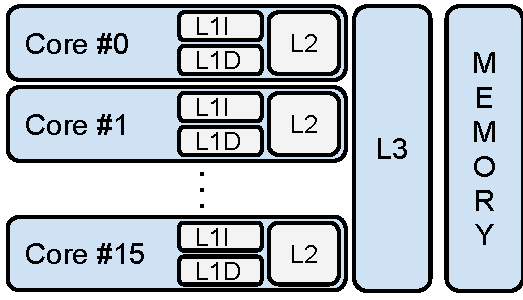
\includegraphics[scale=.65]{figures/processor_model}
\caption{Processor model architecture.}
\label{fig:processor_model}
\end{figure}


\begin{table}[ht]
\centering
\begin{tabular}{rl}
\toprule
\bf{Processor core}                 & 3GHz, OOO, 6 inst. dispatch width,     \\
                                    & 128 rob entries, 4 inst. commit width, \\
                                    & 3 Int. ALU, 1 FP MUL/DIV, 1 FP ADD, \\
                                    & 2 Int. SSE ALU, 1 Int. SSE MUL \\
\bf{Private L1 inst.}               & 32kB, 64B block-size, 4-way, 8 MSHRs, \\
									& LRU, Tag/Data 1/1 cycles \\
\bf{Private L1 data}                & 32kB, 64B block-size, 8-way, 8 MSHRs, \\
									& LRU, Tag/Data 1/2 cycles \\
\bf{Private L2 unified cache}       & 128kB, 64B block-size, 8-way, \\
                                    & 12 MSHRs, LRU, Tag/Data 1/2 cycles     \\
\bf{Shared L3 cache}                & 4/8/16MB, 64B block-size, 24 MSHRs, \\
                                    & 32-way, varying replacement algorithm \\
                                    & Tag/Data 2/5, 2/6, 3/7, 3/9 cycles         \\
\bf{Memory controller}              & 6.4GB/s, 100ns access latency         \\
\bf{Clock Skew}                     & 100 cycle barrier synchronization        \\
\bottomrule                             
\end{tabular}
\caption{Model properties.}
\label{tbl:processor_model:properties}
\end{table}

In this paper, we model a CMP model with two levels of private cache and a shared third layer.
This model is simulated using the Sniper~\cite{Carlson2011} simulation system.
An overview of the system is shown in Figure~\ref{fig:processor_model}, and Table~\ref{tbl:processor_model:properties} lists the system properties.

We are using the Nehalem core model in Sniper and have selected our processor core properties and first level cache size based on the original Intel Nehalem~\cite{Thomadakis2011}. 
We do note that in more recent architectures such as Intel's Haswell~\cite{Jain2013} the core properties have changed compared to the older Nehalem, but the size of the first level cache remains the same.
The reason being that with increasing cache size the access latency increases making it cache unable to feed the processor pipeline with a sufficient stream of instructions and data.

For 4-, 8- and 16-core simulations we will respectively use a 4MB, 8MB, and 16MB L3 configuration.
CACTI~\cite{cacti4} is used to estimate cache latencies for all cache levels.
We configure CACTI to use high-performance storage cells and optimize towards lower access latencies.

\subsection{Benchmarks and Workloads}
\label{sec:methodology:benchmarks}
In all our experiments, we are utilizing benchmarks from the SPEC CPU2006~\cite{SPECCPU2006} benchmark suite. 
We use SimPoint~\cite{simpoint30} to extract 250M instruction intervals from each benchmark that we use in all experiments.
By only extracting a single interval we are willingly increasing the error~\cite{Hamerly2004} between our interval and the results obtained by simulating the entire benchmark.
In our experiments, we are interested in observing performance change in our simulated intervals due to architectural changes.
Producing results comparable to the results of the full benchmark run is not required to achieve this.
Also, it is not obvious how to correctly combine performance metrics used in this thesis from multiple simulated intervals.
Therefore, we choose to use only one interval per benchmark.

We classify each interval based on its sensitivity to changes in available cache space and memory bandwidth.
Based on these classifications we group all benchmarks into one of the following groups:
\begin{itemize}
\item \textbf{Cache sensitive} (ca) benchmarks are in general benchmarks with memory access patterns that are recency-friendly. 

\item \textbf{Bandwidth sensitive} (bw) are benchmarks with no to little temporal locality, often streaming access patterns. 

\item \textbf{Cache- and Bandwidth sensitive} (cabw) are benchmarks with trashing memory access patterns that will benefit from more cache (less trashing) and more bandwidth (faster loading of previously trashed data).

\item \textbf{Compute sensitive} (co) are benchmarks limited by the processing power of the simulated processor.
\end{itemize}
Based on these classifications we generated 4, 8 and 16 core workloads.
The 4 core workloads come in five classes.
One class per benchmark group, these contain workloads only from that particular group.
Also, one class with benchmarks picked from all groups.
The ca and cabw groups contain 5 workloads while the bw and co groups contain 10 workloads.
There is only a single class of 8 and 16 core workloads, as there are not enough benchmarks per group to make workloads of this size. 
The ten 8 and 16 core workloads contain benchmarks from across all benchmark groups.

\subsection{Metrics}
\label{sec:methodology:metrics}
We utilize two metrics to measure the effect of destructive interference between benchmarks in multicore simulations.
System Throughput (STP)~\cite{Eeckhout2010} and the Hamonic Mean of Speedups (HMS)~\cite{Eeckhout2010}.

Two concepts are needed to define these metrics; private mode execution time and shared mode execution time.
Shared mode execution time is the simulation time of a benchmark when run as a part of a workload.
Private mode execution time is the simulation time of a benchmark when run alone on the same processor model.
By definition, we expect a benchmark to execute slower in shared mode than in private mode.

Based on private and shared mode execution time we can define Normalized Progress (NP), or speedup, as ${NP}_i = \frac{T^{P}_i}{T^{S}_i}$.
Here $T^{P}_i$ and $T^{S}_i$ is respectively the private and shared mode execution time for benchmark $i$.
Normalized progress is a measure of benchmark progression in shared mode.
STP is defined by L. Eeckhout~\cite{Eeckhout2010} as the sum of NP for all benchmarks in a workload, as shown in Equation~\ref{eq:STP}.

\begin{equation} \label{eq:STP} 
 {STP} = {\sum\limits_{n=1}^{k}}\frac{T^{P}_i}{T^{S}_i}
\end{equation}

We also define HMS as the harmonic mean of NP values, as shown in Equation~\ref{eq:HMS}.
The summation kernel in HMS is also known as Normalized Turnaround Time (NTT).
HMS is therefore by definition the reciprocal of Average Normalized Turnaround Time (ANTT)~\cite{Eeckhout2010}, and hence HMS has a system level meaning relating to the benchmark's average normalized turnaround-time.

\begin{equation} \label{eq:HMS}
 {HMS} = \frac{k}{{\sum\limits_{n=1}^{k}\frac{1}{\frac{T^{P}_i}{T^{S}_i}}}} = \frac{k}{{\sum\limits_{n=1}^{k}\frac{T^{S}_i}{T^{P}_i}}}
\end{equation}

Finally, we measure cache misses per kilo instruction, MPKI, for all experiments.

\section{Results}

\runar{Add your experiments, condensed}

\section{Related Work}

\toni{Dense discussion of works we did not cover earlier. (Do we even need this section?)}

\section{Conclusion}

\magnus{Write conclusion}